\date{\vspace*{-0.2in}}

%%%\renewcommand{\baselinestretch}{2}
\documentclass[10pt]{sigplanconf}
\nocaptionrule


\newcommand{\footnotenonumber}[1]{{\def\thempfn{}\footnotetext{\small #1}}}
\usepackage[normalem]{ulem}
\usepackage{graphicx}
\usepackage{times}
\usepackage{subfigure}
\usepackage{url}
\urlstyle{rm}

\usepackage{color}
\usepackage{listings}
\usepackage{amsmath}
\usepackage{amsfonts}
\usepackage{amssymb}
\usepackage{comment} 
\usepackage{setspace}
\singlespacing
%\onehalfspacing
\newtheorem{thm}{Theorem}
\newtheorem{prop}[thm]{Proposition}
\newtheorem{cor}[thm]{Corollary}
\newtheorem{lem}[thm]{Lemma}
\newtheorem{defn}[thm]{Definition}


\newcommand{\cfunction}[1]{{\bf \tt #1}}
\newcommand{\malloc}{\cfunction{malloc}}
\newcommand{\realloc}{\cfunction{realloc}}
\newcommand{\free}{\cfunction{free}}
\newcommand{\madvise}{\cfunction{madvise}}
\newcommand{\brk}{\cfunction{brk}}
\newcommand{\sbrk}{\cfunction{sbrk}}
\newcommand{\mmap}{\cfunction{mmap}}
\newcommand{\munmap}{\cfunction{munmap}}
\newcommand{\mprotect}{\cfunction{mprotect}}
\newcommand{\mlock}{\cfunction{mlock}}

\hyphenation{app-li-ca-tion}
\hyphenation{Die-Hard}
\hyphenation{Archi-pe-la-go}
\hyphenation{buf-fer}

\lstset{language=c++, basicstyle=\small\ttfamily,frame=single,tabsize=4}

\definecolor{Gray}{cmyk}{0,0,0,0.5}

\begin{document}

%\renewcommand{\baselinestretch}{2}

\conferenceinfo{XXXXXXXXXXXXXXXXXXX}

\title{Sheriff: Detecting and Eliminating False Sharing}

\authorinfo{}

%Tongping~Liu \and Emery~D.~Berger}
%{Dept.\ of Computer Science \\ University of Massachusetts, Amherst \\
%Amherst, MA 01003} {\{tonyliu,emery\}@cs.umass.edu}

\maketitle

\begin{comment}
%%%%%%%%%%%%%%%%%%%%%%%%%%%%%%%%%%%%%%%%%%%%%%%%%%%%%%%%%%%%%%%%%%%%%%%%%%%%%%%%%%%%%%%%%%%%%
Story:
Multi-core processors or NUMA are now widely used in order to avoid the physical limits of hardware. 
Multi-threaded is considered as one way to take full advantage of those computation resources. Unfornately, 
writing efficient multi-threaded program is not an easy task; 
false sharing problem can reduce the performance greatly, 
even worse, one program with serious false sharing problem can run slower on multi-core machine that that on 
on single-core machine with the same cpu frequency of every core.

This paper presents Sheriff, a system to detect those false sharing problem in multi-threaded c/c++ programs. 
Comparing to previous tool, Sheriff has a very low performance overhead, 
averagely the performance overhead is about 15\% in our experiments. 
For most programs, Sheriff can run almost the same speed or even faster than original program
using pthreads library. 
The second advantage of Sheriff is that there is no false positives at all. 
The false sharing problems reported by Sheriff are actual false sharing problems.

The third adanvatage of Sheriff is that Sheriff can pinpoint the code to cause the false sharing problems. 
For heap objects, Sheriff can point out the allocation site, 
then it is easy for programmer to fix the false sharing problem given the callsite information,
even for some one that are not familiar with the code. 
For global objects, Sheriff can point out those objects' name and length information which has false sharing problem.

How Sheriff to do that?
First, we are using a runtime system which maintains the semantics of multi-threaded program.
To detect those modifications by different threads, we turn those multi-threaded program into a 
multi-process program and use the page protection mechanism to capture those writes on different threads.
In order to capture those writes of different memory, we introduce a "twin" page in the page fault handler;
then we utilize the lazy differentiating mechanism (which has been widely used in distributed share memory) to 
find acutal writes in each phase. 
In order to capture those cache invalidation of different threads, we maintain a global array which is used to
maintain the last thread id to write on one cache line. We use a 
conservative mechanism to count those invalidation of cache lines, 
only those interleaving writes by different threads are counted as an invalidation of corresponding cache line. 
In order to differentiate the false sharing problem from true sharing problem, 
we also keep a word-based version number array 
which is used to record every writes information on each word, including thread id and version. (We use a special
id to identify multi-threads on one word).
 
Also, this word-based versioning mechanism
can help us to the precisely locate the object that are causing the problem if multiple objects are located in 
the same physical cache line.

In order to catch those false sharing problem caused by long transaction, 
we introduce one "sampling mechanism" which can get continutive writes of different threads.

In order to pingpoint the allocation site, we will attach the callsite information for those allocation. Then we can present those callsite when we find out much invalidation. 
 
What else Sheriff can do?
First, Sheriff can work as a run-time system, which can tolerate some of the false sharing problems. 
Second, Sheriff can work as a system which can detect those race condition problems undetectable using those lock-set based tool.
Third, Sheriff can also work as a system to tolerate race problem, like Isolator.

Future work:
(1) Pinpoint the line number to access the cache line by using the "watch point" technique.
(2) Figure out the problem caused by read-write false sharing problem by using the "watch point" technique.
(3) Design a run-time system which can tolerate the false sharing problem in a very low overhead. Profiling 
on specified input should be very helpful to find the problem.
%%%%%%%%%%%%%%%%%%%%%%%%%%%%%%%%%%%%%%%%%%%%%%%%%%%%%%%%%%%%%%%%%%%%%%%%%%%%%%%%%%%%%%%%%%%%%
\end{comment}

\begin{abstract}
Dynamic analysis can be helpful for debugging, but is often too
expensive to use in deployed applications. We introduce evidence-based
dynamic analysis, an approach that enables extremely lightweight
analyses for an important class of errors: those that can be forced to
leave evidence of their existence. Evidence-based dynamic analysis lets
execution proceed at full speed until the end of an epoch. It then
examines program state to find evidence that an error occurred at some
time during that epoch. If so, execution is rolled back and
re-execution proceeds with instrumentation activated to pinpoint the
error. We present \doubletake{}, a prototype evidence-based dynamic
analysis framework. We demonstrate its generality by building analyses
to find buffer overflows, memory use-after-free errors, and memory
leaks. \doubletake{} is precise and efficient: its buffer overflow
analysis runs with just 2\% overhead on average, making it the fastest
such system to date.


\end{abstract}

\terms
Performance, False sharing

\keywords
Concurrency, False Sharing, Performance, Multi-threaded program

%%%%%%%%%%%%%%%%%%%%%%%%%%%%%%%%%%%%%%%%%%%%%%%%%%%%%%%%%%%%%%%%%%%%%%%%%%%%%%%%%%%%%%%%%%%%%
%%%%%%%%%%%%%%%%%%%%%%%%%%%%%%%%%%%%%%%%%%%%%%%%%%%%%%%%%%%%%%%%%%%%%%%%%%%%%%%%%%%%%%%%%%%%%

\section{Introduction}
For decades, applications enjoyed automatic and regular performance gains from increasingly faster CPU speed.  However, this trend has stopped permanently because of hard physical limits. Increasing CPU speed results in consuming more energy and generating more heat. Intel and other vendors have turned to providing more and more cores on a single machine, which brings us the multi-core era. The appearance of multi-core drives the biggest revolution multithreaded programs of software development: software has to be programmed in a concurrent and parallel way in order to exploit the benefits of multi-core machines.

Building efficient and reliable concurrent software is still a challenging task because of the following reasons. First, concurrency requires programmers to think in an unnatural way that humans find difficult.  Second, existing languages and tools are inadequate to detect or prevent concurrency errors and performance anomalies. 

% Why we need determinism? Concurrency errors?
Concurrency errors of multithreaded programs, such as race conditions, atomicity violations, order violations and deadlocks, are very hard to debug ~\cite{Lu:2008:LMC:1346281.1346323}, because their occurrences highly depend on some specific conditions, such as thread interleavings and CPU scheduling ~\cite{DBLP:conf/icse/BallBHMQ09,DBLP:conf/asplos/BurckhardtKMN10}. Instead of detecting possible concurrency errors, one promising alternative approach is to attack the problem of concurrency bugs by eliminating its source: non-determinism. A fully \emph{deterministic multithreading system} would prevent Heisenbugs by ensuring that executions of the same program with the same inputs always yield the same results, even in the face of race conditions in the code. Such a system would not only dramatically simplify debugging of concurrent
programs~\cite{Carver:1991:RTC:624586.625040} and reduce their attendant testing overhead, but would also enable a number of other applications. For example, a deterministic multithreaded system would greatly simplify record-and-replay for multithreaded programs~\cite{Choi:1998:DRJ:281035.281041,LeBlanc:1987:DPP:32387.32396} and the deterministic replication of a multithreaded application on different machines for fault tolerance~\cite{deterministic-process-groups,1134000,224058,replicant-hotos}.

% Why we need to find out false sharing problems.
Besides concurrency errors, writing efficient multithreaded programs remains challenging too. False sharing problem is one of the notorious performance problems inside multithreaded programs~\cite{falseshare:Analysis, falseshare:effect}. It occurs when multiple threads, running on different cores with their separate caches, are accessing logically independent words in the same cache line. If a thread modifies anything inside a cache line, cache coherence protocol invalidates the duplicates of this cache line in other caches in order to guarantee correctness of programs, which is crucial for true sharing cases. However, it is totally unnecessary for false sharing cases. False sharing can force one core to wait unnecessarily for updates from another processor, thus wasting both the CPU time and precious memory bandwidth in the same time. 

\subsection*{Contributions}

This thesis handles two categories of problems inside multithreaded programs, the reliability problem and the performance problem, and makes the following contributions:

\begin{itemize}
\item \Sheriff{} framework: I developed a novel processes-as-threads framework by borrowing the idea from Grace~\cite{grace}. \sheriff{} is a software-only drop-in replacement of the stand \pthreads{} library. It turns threads into processes, with separate address spaces but the shared file table. \sheriff{} provides per-thread memory protection and isolation on page granularity, relying on the stand memory protection mechanism and twining-and-diffing mechanism. \sheriff{} enables a range of possible applications, including language support and enforcement of data sharing, software transactional memory, thread-level speculation, and race detection. 

\item I developed an efficient deterministic multithreading system, \dthreads{}, for unmodified C/C++ applications,  without programmer intervention and hardware support. \dthreads{} is based on the \sheriff{} framework to isolate executions of different threads. \dthreads{} outperforms the previous state-of-the-art runtime system (CoreDet) by a factor of 3, and often matches and sometimes exceeds the performance with the standard \pthreads{} library. \Dthreads{} enforces robust/stable determinism even in the face of data races, greatly simplifying program understanding and debugging: programs always behave the same, even with different inputs and on different hardware, as long as the synchronization order is staying the same. Because of this, \dthreads{} can also be used to support replicated executions of multithreaded applications for fault tolerance purposes.

\item 
Based on the \sheriff{} framework, I developed another two tools, \SheriffDetect{} and \SheriffProtect{}, to deal with false sharing problems of multithreaded programs, one of the notorious performance problems. 
\SheriffDetect{} find instances of false sharing accurately (no false positives), runs with low overhead (on average 20\%), and can precisely pinpoint the exact objects involved in false sharing. \SheriffProtect{} mitigates false sharing problems by adaptively isolating shared accesses on a cache line from different threads into separate physical addresses, effectively eliminating the performance impact of false sharing. It can boost the performance automatically for those multithreaded applications with false sharing problems inside, without the need of programmer intervention. 

\item I also developed a tool, \predator{}, to improve the effectiveness of false sharing detection. Instead of relying on the \sheriff{} framework to track memory writes, \predator{} employs compiler instrumentation to track read and write memory accesses, which make it possible to detect one more type of false sharing, read-write false sharing. \Predator{} also overcomes a key limitation of previous detection tools: existing tools can only detect those observed false sharing problems. However, the occurrences of false sharing highly depend on memory layout and size of a cache line, which are affected by a lot of dynamic properties. \Predator{} can predict potential false sharing that does not manifest in a given execution but may appear---and greatly degrade application performance—--in a slightly different execution environment. \Predator{} is the first false sharing tool able to automatically and precisely uncover false sharing problems in real applications, including MySQL and the Boost library.


\end{itemize}

\subsection*{Outline}
The rest of this thesis is organized as follows. Chapter~\ref{chapter:problems} describes the reliability and performance problems of multithreaded programs, which we are going to handle in this thesis. Chapter~\ref{sec:sheriffframework} describes the processes-as-threads framework, \sheriff{}, which is the basis for \dthreads{}, \SheriffDetect{} and \SheriffProtect{}. Chapter~\ref{chapter:dthreads} describes \dthreads{} that ensures deterministic execution for multithreaded programs linking to this drop-in library. Chapter~\ref{chapter:sherifftools} discusses how to precisely detect and automatically tolerate false sharing problems based on the \sheriff{} framework. Chapter~\ref{chapter:preditor} describes a generalized false sharing detection tool by combining compiler instrumentation and runtime system, which improves the effectiveness of false sharing detection. 
Chapter~\ref{chapter:relatedwork} provides a substantial comparison between previous work and our approaches and Chapter~\ref{chapter:conclusion} concludes the thesis with its contributions and possible future work. 


%%
%% Some sample text




\section{Sheriff Overview}
Figure~\ref{fig:nondeterminism} shows an example multithreaded program that, because of data races, non-deterministically produces the outputs ``1,0,'' ``0,1,'' and ``1,1.''  The order of instructions are changed from one execution to the other, resulting in these nondeterministic outputs. Using \dthreads{}, this program will \emph{deterministically} produce the same output-``1,1'' . Although this output can be a undesired one, the fact that results are always reproducible would make it easy for developers to reproduce and locate data races inside parallel programs.

\begin{figure}[h]
{\centering
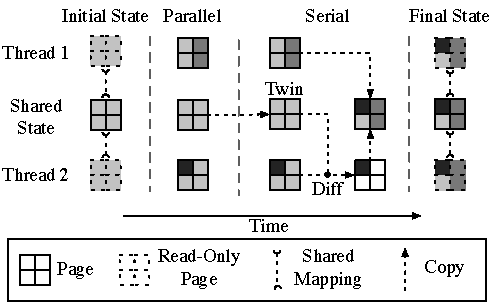
\includegraphics[width=6in]{dthreads/figure/architecture-diagram}
\caption{An overview of \dthreads{} execution.\label{fig:architecture}}
}
\end{figure}

\dthreads{} employs the following mechanisms to ensure the deterministic execution, illustrated by Figure~\ref{fig:architecture}: 

\textbf{Isolated Memory Access:} In \dthreads{}, threads are actually running as separate processes with private and shared views of memory, which is based on the \sheriff{} framework. Because processes have separate address spaces, \dthreads{} can isolate executions of different ``threads''. \dthreads{} uses this isolation mechanism to control the visibility of memory state, so that the updates made by a thread can not be seen by other threads if those updates are not committed explicitly to the shared mapping. By doing this, we guarantee that each ``thread'' can operate independently until synchronization points. Implementation of this is discussed in depth in Section~\ref{sec:threadsasprocs}.

\textbf{Deterministic Memory Commit:} 
Multithreading programs use shared memory for communication, thus \dthreads{} must propagate a thread's changes to be seen by other threads. To guarantee determinism, \dthreads{} should publish updates of different threads in a deterministic order at deterministic points.

\dthreads{} actually commits the changes of a thread to the shared state in sequence at synchronization points. These points includes thread creation and exit; mutex lock and unlock; condition variable wait and signal; posix sigwait and signal; and barrier waits. Commits are ordered using a global ``token'' that is passed from one thread to the next; a thread can only commit when it holds the token.  The token-passing protocol is described in Section~\ref{sec:schedule} and the implementation of synchronization primitives is described in Section~\ref{sec:synchronization}.

\dthreads{} relies on the twinning and diffing mechanism to find out local changes of different threads, which has been discussed in Section~\ref{sec:twinning-and-diffing}. 

\textbf{Deterministic Synchronization:}
There is no deterministic guarantee on synchronizations under existing operating systems. Thus, \dthreads{} re-implements the full range of pthreads synchronization primitives and discusses  them in details in Section~\ref{sec:synchronization}. 

\hspace{1em} \\
\noindent
\textbf{Fixing the data race example} \\
About the example program in Figure~\ref{fig:nondeterminism},  \dthreads{} effectively isolates the execution from each thread until it completes, and then orders updates from different threads by thread creation time using a deterministic last-writer-wins protocol.

In the beginning of every execution, thread 1 and thread 2 have the same view of shared state, with a = 0 and b = 0. Because changes by one thread to the value of a or b will not be made visible to the other until this thread exits, both checks on two threads on line 2 will be true. Thread 1 sets the value of a to 1, and thread 2 sets the value of b to 1. These threads then commit their updates to the shared state and exit, with thread 1 always committing before thread 2. The main thread then should always prints “1, 1” on every execution.

This determinism not only enables record-and-replay and replicated execution, but also effectively converts Heisenbugs into “Bohr” bugs, making them reproducible. In addition, \dthreads{} optionally reports any conflicting updates due to racy writes, further simplifying debugging.


\section{Simulation of multi-threaded program}
\label{sec:simulation}

This section we are going to talk how to replace threads with processes while still maintain
the same semantics of multithreaded program.

We are going to answer the following questions in the following subsections:
\begin{itemize}
\item How to turn threads into proceses? 
\item How to maintain the semantics to share the same address space?
\item How to share file access?
\item How to handle synchronization among threads?
\end{itemize} 

In the end, we are going to talk how to simuate the threads in one phase.
\subsection{Thread Creation and Exit}
Sheriff intercepts those function calls of \texttt{pthread\_create()} then replaced that with a \texttt{fork()} system call.
Child processes invokes the routine passed by \texttt{pthread\_create()} calls. 
In this way, Sheriff fork off new processes instead. 

Sheriff use one explicit \texttt{\_exit()} call to terminal current thread.

\subsection{Share Address Space}
\label{simulation:sharememory}
In order to create the illusion of multi-threaded programs that 
different threads are sharing the same address space, 
Sheriff uses the memory mapped files to share the heap and globals across different processes.
It is noted that Sheriff don't try to share the stack across different processes 
because different threads have their own stacks and 
it is un-common to use stack to communicate between different threads.

Sheriff creates two different mappings for both the heap and the globals. 
One is shared mapping, which is working as a backstore using to hold those shared state. 
Another one is private, copy-on-write(COW) mapping (per-process) that each process works on directly.
Private working mapping are connecting to the shared mapping through the one memory mapped file.

Read/write operations are worked only on private working mappings. 
But actually reads or writes on one page have different effects that depending on the state of one page.
For reads on those pages without private copies, 
reads are actually accessing those pages in the shared mapping dirtectly with the help of memory mapped file.
For reads on those pages with private copies, 
reads can only access those private copies which are guranteed by the separation mechanism of process. 
Writes have one different senario. Private working mapping are setted to read-only mode in the beginning. 
First write on one read-only page can invoke a COW operation that can copy the content from 
corresponding shared mapping. 
After than, user program can only access those private mapping. 
It is the duty of Sheriff to commit those changes
of different processes to the shared mapping in the transaction end (more deatails can be seen in
section~\ref{simulation:thread}.

The details to create the memory mappings for globals and heap are described in the following.
\par\vspace{3mm}
\noindent
\textbf{Globals}
\par\vspace{3mm}
\noindent
Sheriff uses a fixed-size(larger than normal globals size) file to hold globals. Sheriff checks the size of actual
globals to guarantee that the specified size is enough to hold all globals, if not, Sheriff can report this anomaly and 
user can fix that easily.
Sheriff tries to get the start and size of globals for one program and uses \texttt{mmap()} to create a shared mapping 
among different threads. That is, user program are still using the address after the compilation.
Since some global variables may has some initialized value, Sheriff copies all contents 
from the private mapping to the shared mapping. 

\par\vspace{3mm}
\noindent
\textbf{Heap}
\par\vspace{3mm}
\noindent
Sheriff also uses a fixed-size mapping to hold the heap for user application, currently we are using 1.6GB. Memory allocations 
requirements from user applications are met from this fixed-size private mapping.

Since different threads can get the memory from this fixed-size mapping, the heap data structure are shared among different
threads and allocations are protected by one process-based mutex.
In order to avoid the false sharing problems brought by the memory allocator, 
Sheriff builds a scalable ``per-thread'' heap organization that is loosely based on Hoard~\cite{BergerMcKinleyBlumofeWilson:ASPLOS2000} and built using HeapLayers~\cite{BergerZornMcKinley:2001}. 
Sheriff divides the heap into a fixed number of sub-heaps(currently 16). Each thread uses a hash of its process id to obtain
the index of the heap which can be used to satisfy memory allocations. 
This origranization has two benefits. First, it can minimize the conflicts caused by using only 
one shared heap between different threads, thus avoiding the performance impact by using the lock to 
maintain the data consistency.
Second, it avoids the false sharing problems caused by heap objects. Since each thread are using different pages 
to satisfy memory allocations, objects allocated by one thread has no chance to be the same 
cache line with objects from another thread. Thus, runtime system build on that can avoid false sharing problems 
and have a much better scalability. 

\begin{comment}
Not all memory allocations are meet from the protected heap to avoid the performance problem. 
Since those accesses on protected heap, the first write on each transaction should pay the overhead to 
create the copies and later should do the comparison and commit in the end of transaction.
Those overhead is additional comparing to normal running of multi-threaded program. 
We believe that false sharing problem has a greater chance to happen in those small allocations (smaller than cores number 
times of cache line size). Huge block of memory normally is not a source of false sharing problem. 
Besides those mapping to work as a shared backstore and a working copy, Sheriff provides an additional MAP\_SHARED mapping 
which is used to meet the allocation requirements of larger objects.
\end{comment}

\subsection{Share File Access}
\label{sec:fileshare}
\begin{figure}[!t]
\small
\begin{lstlisting}[frame=trbl]{}
int spawnWithShareFiles{
  return syscall(SYS_clone, 
   CLONE_FS|CLONE_FILES|SIGCHLD,(void*)0);
}
\end{lstlisting}
\caption{Pseudo-code to create a new process.
\label{fig:newfork}}
\end{figure}
In multi-threaded programs, different threads in the same process share opened files of each thread. 
But multi-processes is a different senario: 
each process is assumed to own all of its resources, including memory, file handles, sockets, device handles, and windows. 

Since Sheriff tries to approximate the semantics of multi-threaded programs.
it is necessary to make different processes to share opened files.
One naiive way is to create a process to work as the proxy for other processes, this proxy can \texttt{open/close} files 
or change attributes of files for other processes. 
After that, the proxy can use a ``Unix domain socket'' to pass the descriptor from the proxy to the initiating process 
and other processes wanting to share this file ~\cite{passfd}. 
But it is not easy to do this since we have to wrap up a lot of file system related system calls. 
Also, there is some additonal overhead of communication.

Sheriff uses a different approach, by setting the flag \texttt{CLONE\_FILES} 
when creating new processes (Fig.~\ref{fig:newfork}), 
child processes can share the same physical file descriptor table with the parent process. 
Then Sheriff can share files among different processes.
\begin{comment}
It is noted that using \texttt{clone()} to create new process will affect the getpid() system call.
Although current thread model is the 1-to-1 model in pthreads library (not n-to-1 model any more), 
glibc's wrapper will always return the process ID of the parent process via the glibc wrapper function. 
Sheriff avoid this predicament by intercept getpid() calls then just give the stored pid for different threads.
\end{comment}

\subsection{Synchronization}
\label{simulation:syn}

\begin{figure}[!t]
\small
\begin{lstlisting}[frame=trbl]{}
  void sync(var) {
    closeTransaction();

	realVar = getRealVariable(var);
	pthread_sync(realVar);
	
    startTransaction();
  }
\end{lstlisting}
\caption{Pseudo-code for all synchronization operations.\label{fig:synccode}}
\end{figure}
Synchronization are used to coordinate the activities and data accesses among different threads. 
Synchronization also means that some shared data needs to be changed or be used across different threads. 
For example, program calls \texttt{mutex\_lock()} when it needs to access some shared data. 
There are some \textbf{synchronization} mechanisms in multithreaded program, 
including: \textit{mutex}, \textit{conditional variable}, \textit{barrier} and \textit{join}.

In order to describe things easier, we introduce the ``transaction'' concept here. 
``transaction'' is used to describe one piece of code which executes in a atomical,  
separated and consistent way. 
It is noted that Sheriff is not one traditional transactional memory system.
Transaction Memory is a concurrency control mechanism 
attempting to simplify the parallel programming by allowing a group of instructions 
to execute in an atomic way.
Traditional transaction memory systems are optimized for short transactions,
but do not effectively support long-lived transactions. They also provides a rollback mechanism
when one transaction fails to commit. 
Sheriff won't support rollback here and supports any length of transaction, 
longer transaction is better to amortize the overhead,
and tends to use for general multi-threaded program, 
no need to annotate the code as ``transaction'' manually.
Also, Sheriff don't replace the lock usage as some log-based mechanism.
But transaction concept in Sheriff has the atomicity, isolation and consistency attributes, which is 
the same as that in transactional memory~\cite{transaction}. 

\begin{comment}
Sheriff read-protects all pages of memory in the beginning of memory so that any intends to write on one 
page can be captured by Sheriff by handling the page fault. 
In the end of transaction, Sheriff tries to publish the modifications
made by current transaction so that other threads in the same application can see the modifications by one thread.
\end{comment}

In order to simulate those multithreaded synchronization, Sheriff intercepts those synchronization object 
initialization function calls, allocates one new synchronization object on a shared mapping (shared by all processes)
and initializes them to be accessed by different processes. Then the new object's address can be saved 
in the header of original object. 
Handling about one synchronization call can be seen in Fig.~\ref{fig:synccode}. 

In order to explain it more clear, we are using the mutex as an example. There are three regions for one mutex usage: 
the first region is before \texttt{mutex\_lock}; the second region is between \texttt{mutex\_lock} and \texttt{mutex\_unlock}; 
 the third region is after \texttt{mutex\_unlock}. Sheriff chooses to use three different transactions for these three different regions.
Although it is unnecessary to do so for the first and third region since they don't need 
to executed in a atomical and isolated way. But it is better to do so for easiness.

For the first and third region, introduction of transaction here won't cause correctness problem 
according to Sheriff's assumption(Section~\ref{overview:assumption}). Other threads are not supposed 
to access the data modified by current process.

For the second region, when there is \texttt{mutex\_lock} and \texttt{mutex\_unlock} call, 
Sheriff are trying to call corresponding
pthreads library's functions but worked on a process-based mutex object. 
According to the semantics of multithreaded program, the modifications happening between \texttt{mutex\_lock} 
and \texttt{mutex\_unlock}
are unseen by other threads and modifications can work on shared memory directly (it is also safe to so).  
In actual implementation, it is relatively expensive to 
change page mapping between \texttt{MAP\_SHARED} and \texttt{MAP\_PRIVATE} 
especially when the memory footprint is very large. To avoid those unnecessary overhead, 
Sheriff starts a new transaction after \texttt{mutex\_lock()} and closes that transaction in case of \texttt{mutex\_unlock()}. 

For conditional variable and barrier, they are using the same mechanism as the example in Fig.~\ref{fig:synccode}.
\texttt{pthread\_join} is a little different. Sheriff just closes current transaction and calls \texttt{waitpid()} 
when there is a \texttt{pthread\_join()} call. 

\subsection{Thread Execution}
\label{simulation:thread}
As what we described above, Sheriff uses the transaction(atomic execution) to simulate 
those synchronization mechanism of multithreaded program. 
The overview of this mechanism can also be seen in Fig.~\ref{fig:overview}.
 
Before the program begins, Sheriff establishes shared and local mappings for the heap and globals. 
\begin{comment}
To improve the performance, Sheriff don't do page protection when there is just one thread; read/write operations
work on shared mappings directly to avoid protection overhead and commit overhead. 
We implement this in the following two cases:
First, Sheriff will start page protection until there is a pthread\_create() function call  
to spawn one child. 
Second, Sheriff will close page protection when there is just one thread.
Sheriff always checks whether current thread is the only thread in the system in pthread\_join() function
and close the page protection timely if it is.

To start the protection, those pages in the protection range will be set to MAP\_PRIVATE and PROT\_READ mode; 
later access on one protected page should invoke a Copy-On-Write operation in the operating system.
To stop the protection, those pages in the protection range will be re-set to MAP\_SHARED and readable/writable; later access 
access on those pages will work on shared mapping directly(through mapping file). 
\end{comment}
\subsubsection{Transaction Begin}
In the beginning of one transaction, Sheriff sets every page in the protection range to \texttt{PROT\_READ} so that
later writes on those pages can be caught by handling \texttt{SEGV} protection faults.
In fact, Sheriff don't need to set on every page, only those pages dirtied in last transaction needs to be
set to \texttt{PROT\_READ}; other clean pages should still in the \texttt{PROT\_READ} 
since the mode bit of those pages are kept the same
in the execution if one page is not modified.

Sheriff clears dirty pages sets after it set every dirty page to \texttt{PROT\_READ}.

\subsubsection{Execution}
\label{simulation:execution}
When no page under protection is written, Sheriff runs almost the same speed as that of multithreaded program. 
When those pages under protection are written, that triggers a page fault and Sheriff can
be involved in by handling \texttt{SEGV} protection faults.
 
The algorithm of page fault handler is listed in the following:
\begin{enumerate}
\item 
Sheriff tries to get the page holding the faulted address and then set this page to write-able so that 
future accesses on this page can run at a full speed (won't invoke page fault any more). 
Thus, one page incurs only one page fault in one transaction. 
Although protection faults and signal faults are expensive, those cost 
can be amoritized for the whole transaction.

\item 
Before the creation of ``twin page'', Sheriff force a Copy-On-Write operation on this page by writing to the start of this page 
with the content getting from the same address. 
This step is very important to get two identical pages for ``twin'' page and working copy 
so that comparison of those two can give actual modifications made by this transaction. 
Since there is a time gap between the creation of ``twin'' pages and that of ``private'' pages, private pages are created 
by OS's COW after the signal handler. 
After the force of a COW, Sheriff creates a copy of current page from share area to a local store(called as ``twin'' page). 
This ``twin'' page mechanism has been discussed in Section~\ref{overview-twinpage}.
\item 
In the end of page fault handler, Sheriff adds page address to the \textit{dirty} set so that 
all dirty pages can be checked in the end of transaction.
\end{enumerate}

\subsubsection{Transaction End}
\label{simulation:endtran}
In the end of each atomically-executed region - the end of each thread, right before and end of those synchronization points, 
right before a thread spawn, and right before joining another thread - 
Sheriff commits those changes from ``private'' pages to ``shared'' mapping, 
then remove those old private pages and twin pages.

Then Sheriff will trying to commit those modifications in current transaction to ``shared'' mapping so that other threads can
see those changes modified by current transaction. 
As what we desribed in Section~\ref{overview-twinpage}, those ``twin'' pages and ``working'' (private) pages
can be compared word by word in order to capture those modifications in current transaction. 
Those new values on ``working'' pages will be committed to the same offsets of corresponding ``shared'' mapping.

After commits, Sheriff issues a madvise (\texttt{MADV\_DONTNEED}) call to discard current physical pages of ``private'' mapping 
. Since Sheriff allocates some physical pages to 
hold those ``twin'' mapping, those pages should be discarded too to avoid the memory leakages. 
Note here that Sheriff will hold a global lock in order to do commits and updations automically. 
\begin{comment}
\begin{figure}[!t]
\small 
\begin{lstlisting}[frame=trbl]{}
//@This function is called by pthread_join
void uniqueChecking (void) {
  // Is it the initial thread?
  if(getpid() == initialPid) {
	// Using waitpid to check the uniqueness.
    if(waitpid(-1, NULL, WNOHANG) == -1 
	   && errno == ECHILD) {
		// Close protetion here.
        closeMemoryProtection();
        _protected = false;
    }
  }
}
\end{lstlisting}
\caption{Pseudo-code for unique checking.\label{fig:unique}}
\end{figure}

\end{comment}


\section{Detection of False Sharing}
\label{sec:falseshare}
From above section, we already know that how to design a runtime system to simulate the running 
of multi-threaded program. 

In this section, we are going to talk how to indentify false sharing problems by recording memory writing using
the runtime system.
This section are trying to answer the following questions:

\begin{itemize}
\item How to capture the memory writes from different process?
\item How to capture the continuous memory writes?
% - sampling mechanism - "temporary twin" and "original twin". 
\item How to capture the interleaving cache invalidation? 
% Use a global array, updating timely when modification is detected. 
\item How to identify objects inside one cache line? 
%Attach the callsite information to capture the allocate sites for heap objects. 
\item How to differentiate true sharing and false sharing?
%detect the combination? An array to get word version and threads working on that. We can detect those fields inside one object causing the problem too.
\item How to report one false sharing problem?
% In the end of program, we traverse the whole global array.
\end{itemize}

\subsection{Capture of Memory Writes}
\label{falseshare:memorywrites}
Process can provide a strong isolation of one thread's running from other threads' running. 
In each transaction, Sheriff runs one thread in a atomical, consistent and isolated way and
won't commit those changes in one transaction until the end of one transaction.
In the end of each transaction, Sheriff can compare ``twin'' page and ``working'' page word by word to find 
those modifications on each dirty page. When the word of ``working'' page is different from that of 
corresponding ``twin'' page, this word is thought to be modified by current thread in current transaction. 
It is reasonable to reach this conclusion since Sheriff can guarantee that originally the content of ``twin'' page 
is the same as that of ``working'' page by forcing a COW explicitely (see ~\ref{simulation:execution}).
\begin{comment}
It is true that the writing of ``A-B-A''  can be missed by simply comparison,
but we believe that ``A-B-A'' writing in one transaction
is not frequent and won't bring any correctness problem.
We don't want to put too much focus on this point.
\end{comment}

Since we can capture the memory writes on every transaction and one thread's running is consisted of multiple transactions, 
we can capture the memory writes from different threads.

\subsection{Capture of Continuous Writes}
\label{detection:sampling}
We already know from above section that Sheriff can capture memory writes on one transaction. 
But it is not good enough when the transaction length is too long (some extreme case can be the whole thread). 
Actually, one serious false sharing problem (\texttt{linear\_regression} benchmark, see Section~\ref{sec:evaluation}) 
which affect the performance 10X can be omitted since there is only one transaction for one thread, 
without any synchronization inside. 

Sheriff use a sampling mechanism to avoid this problem. Sampling is 
to select some of observations in order to acquire some knowledge about the whole.
Although sampling cannot give complete information about memory writes on one transaction,
sampling can be used to capture more writes. More fine sampling can help to find more writes by one transaction.
There is a balance between choosing finer sampling period and performance issue here. 
Sheriff now choose 10 microseconds as a basic interval to do sampling. 

In order to capture continuous writes, Sheriff introduce one ``temporary twin'' page for every shared dirty page
 (see Fig.\ref{fig:overview}). 
Handling of those ``temporary twin'' pages are slightly diferent with those ``original twin'' pages.
First, they are created in the sampling timer handler when one page is found to be shared by multiple threads. 
There is no use to create ``temporary twin'' for those pages only accessed by one thread. We are using a global array to
record users for one page. 
Second, ``temporary twin'' pages are keeping updated to ``working'' version in every timer handler 
in order to capture future writes on the same page.
 
\subsection{Capture of Cache Invalidations}
\label{detection:invalidation}
Just as we talked in Section~\ref{overview:target}, only numerous interleaving writes can bring performance problem. 
Sheriff tries to capture the interleaving writes across different threads in order to capture 
cache invalidations. 

In order to capture interleaving writes on caches, Sheriff introduces 
virtual cache line status words (Fig.~\ref{fig:overview}). 
``virtual'' is used here to differentiate with ``physical'' cache line. 
For every virtual address range (same size with physical cache line) under protection, Sheriff assigns one status word. 
One status word has two fields, the first field points last thread to write on this cache line, 
the second field is used to record times of invalidates (version) on one cache line. 
Every time when one different thread are detected to write on this cache line, Sheriff update both the thread id
to be the new thread and version number. 
In actual implementation, Sheriff introduce two different arrays to avoid using lock. Corresponding code can be seen
in Figure~\ref{fig:capturecacheinvalidation}.
CacheInvalidation array is used to capture those interleaving cache invalidation for all cache lines in protected memory. 
Every cache line have one corresponding counter to indicate the interleaving of cache invalidation for this cache line. 
LastThreadModifyCache array is used to record last thread id to write on its cache line. 

The pseudo code to capture the interleaving cache invalidation is listed in Figure~\ref{fig:capturecacheinvalidation}:
\begin{figure*}[!t]
\begin{lstlisting}
void recordCacheInvalidates(int cacheNo) {
    int myTid = getpid();
    int lastTid;

    // Try to check last thread to modify this cache.
    lastTid = atomic_exchange(&LastThreadModifyCache[cacheNo], myTid);
    if(lastTid != myTid) {
       // Increment cache invalidation only when current thread is different.
       atomic_increment(&cacheInvalidation[cacheNo]);
     }
}
\end{lstlisting}
\caption{Record the cache invalidation atomically.\label{fig:capturecacheinvalidation}}
\end{figure*}

\subsection{Indentify Objects inside Cache Line}
\label{detection:object}
For global object, Sheriff don't need to do anything since debug information can provide
object's information.
Sheriff attaches the call site in the header of each heap object when allocation to indentify objects.
Callsite information can provide objects' request allocation, which is useful for programmer
to fix the false sharing problem (see case study in Section~\ref{evaluation:comparison}).
It is one important feature to differentiate Sheriff from previous tools.
Previous tools using binary instrumentation or hardware performance counter cannot control
the memory allocation, so they cannot provide the callsite information about one object.
Sheriff is a runtime system which intercepts all heap allocations so that Sheriff can tell programmer
about cache line's object information.

Remember that Sheriff have two arrays to capture the cache interleaving invalidation
(see Section~\ref{detection:invalidation}), it is necessary to cleanup those invalid counting
when one object is de-allocated. It is important to avoid the false positives caused by uncorrectly aggregate 
counting when one address is re-used for other objects. 

\subsection{Avoidance of False Positives}
\label{detection:avoidfalsepositive}
To avoid false positives, 
Sheriff introduces another global array to record  
threads writing on each word and version numbers of each word.
Threads writing on each word can tell whether one cache line is false sharing or true sharing. 
Version number on each word can avoid to report those objects which don't contribute much on cache invalidations, 
when there are multiple objects in the same cache line.
In order to save space, Sheriff use one word's higher 16 bit to store the thread id on one word
and use the lower 16 bit to store version number of this word. 
When one word is detected to be modified by more than two threads, we marked specially
on its thread id field.

\subsection{Reporting False Sharing Objects}
In the end of program, Sheriff reports those objects causing false sharing problems. 
Since Sheriff introduce a global array (CacheInvalidationArray) to record those 
cache invalidation (see Section~\ref{detection:invalidation}), Sheriff checks 
CacheInvalidationArray for cache lines with invalidation times larger than one water level. 
After one cache line is found, corresponding invalidation times and offset of this cache line 
will be added into a global link linst sorted by invalidation times. 
Later we can rank the false sharing objects by invalidation times they caused. 

After the traverse of all cache lines, Sheriff tries to get objects information 
for all cache lines in the link list. 
Sheriff uses magic value added in the allocation to differentiate the start of one object. 
Also, the object size information can help to identify the start of one object. 
After finding out those objects inside one cache line, Sheriff should look into the 
array listed in Section~\ref{detection:avoidfalsepositive} to avoid false positives. 

%%%%%%%%%%%%%%%%%%%%%%%%%%%%%%%%%%%%%%%%%%%%%%%%%%%%%%%%%%%%%%%%%%%%%%%%%%%%%
%%%%%%%%%%%%%%%% Where to specify those procedure of timer handler????? LTP
%%%%%%%%%%%%%%%%%%%%%%%%%%%%%%%%%%%%%%%%%%%%%%%%%%%%%%%%%%%%%%%%%%%%%%%


\section{Discussion}
\label{sec:discussion}

\subsection{Instrumentation Selection}
\label{sec:instrumentationtradeoff}
Dynamic binary instrumentation and compiler-based instrumentation are two alternative approaches to perform instrumentation~\cite{Instrumentation}. They exhibit different tradeoffs of performance and generality. Dynamic binary instrumentors, such as Valgrind~\cite{Valgrind}, Pin~\cite{Pin}, and DynamoRIO~\cite{DynamoRIO}, typically analyze the program's code just before execution in order to insert instrumentation. They introduce significant performance overhead, mostly caused by run-time encoding and decoding, but the fact that they operate directly on binaries makes them extremely convenient. By contrast, compiler instrumentation inserts instrumentation in the compilation phase, which requires re-compilation of all source code. 
\Predator{} employs compiler-based instrumentation both because of its better performance and its greater flexibility, as discussed in Section~\ref{sec:selectinstrumentation}.

\subsection{Effectiveness}
Several factors can affect \Predator{}'s ability to identify false sharing.

\emph{Different Inputs.} Different inputs trigger distinct executions of a program. If a specific input does not exercise the code with false sharing problems, \Predator{} cannot necessarily detect them. However, \Predator{} does generalize over inputs to find latent false sharing problems on those exercised code. When any reasonably representative set of inputs are exercised, as is required by any testing regime, \Predator{} can effectively predict false sharing.

\emph{Input Size.} Input size may affect detection results.  As discussed in Section~\ref{optimization}, \Predator{} introduces several threshold values to reduce tracking overhead, which can be adjusted as needed. If the input size is so small that it cannot generate enough false sharing events to cross the pre-defined thresholds, then the detection mechanism will not be triggered. In such cases, \Predator{} will miss actual cases of false sharing. However, realistically large inputs should be enough to trigger \Predator{}'s detection mechanisms. 

\emph{Hardware Independence.}  \Predator{}'s compiler-based approach make it independent of the underlying hardware platform. This approach increases generality, but may lead to over-report false sharing. \Predator{} conservatively assumes that different threads are running on different cores and detects false sharing problems based on possible cache invalidations. However, if multiple threads involved in false sharing are on the same core, then there will be no performance impact. 

%\subsection{Prediction Limitations} 
%\Predator{} can accurately and precisely predict a false sharing problem even when it does not occur. But \Predator{} cannot predict a false sharing problem if the code with false sharing is not exercised at all. Also, \Predator{} may miss potential false sharing problems between two objects brought by a different compiler or memory allocator. 


\section{Evaluation}
\begin{figure*}[htb]
{\centering
\tiny
\subfigure{\lstinputlisting[numbers=none,frame=none,boxpos=t]{predator/figure/linearregression.report}}
\caption{An example report by \Predator{} indicating false sharing in the linear\_regression benchmark.
\label{fig:lrreport}}
}
\end{figure*}



\label{sec:evaluation}

This section answers the following questions:
\begin{itemize}
\item
  How effective is \Predator{} at detecting and predicting false sharing?

\item
  What is \Predator{}'s overhead, in terms of execution time and memory ?

\item
  How sensitive is \Predator{} to different sampling rates?
 
\end{itemize}

\paragraph{Experimental Platform.} All evaluations are performed on a quiescent Intel Core 2 dual-processor system equipped with 
16GB RAM. Each processor is a 4-core 64-bit Intel Xeon running at 2.33 GHz, with a 4MB shared L2 cache and 32KB private L1 cache. The underlying operating system is an unmodified CentOS 5.5, running with Linux kernel version 2.6.18-194.17.1.el5. The glibc version is 2.5. 

\paragraph{Evaluated Applications.}
This paper evaluates two popular benchmark suites,
Phoenix (with large input) ~\cite{phoenix-hpca} and PARSEC (with simlarge input) ~\cite{parsec}. Even with unmodified LLVM-3.2, Facesim cannot be compiled successfully (having complaints on an undefined template) and Canneal aborts unexpectedly. Thus, these two benchmarks are excluded.
We also evaluate \Predator{} on six real applications, including MySQL, Boost, Memcached, aget, pbzip2 and pfscan.



\subsection{Detection and Prediction Effectiveness}
\label{sec:effective}

For every false sharing problem, \Predator{} reports source code information and detailed memory access information in order to help users fix those problems. Figure~\ref{fig:lrreport} shows an example for the linear\_regression benchmark. This report shows that the heap object starting with $0x40000038$ potentially causes a large number of cache invalidations. The call stack of allocation is provided to help locate culprits. In addition, \Predator{} also reports word-level access information of this object, which helps to identify where and how false sharing occurs. From that, we can know that it is a latent false sharing problem predicted by \Predator{}, since different threads are accessing different cache lines. 

\subsubsection{Benchmarks}
\label{sec:benchmarks}

\begin{table*}[!t]
{\centering\begin{tabular}{l|r|r|r|r|r}\hline
{\bf \small Benchmark} & {\bf \small Source Code} & {\bf \small New} & {\bf \small Without Prediction} &{\bf \small With Prediction} & {\bf \small Improvement} \\
\hline
\small \textbf{histogram} & {\small histogram-pthread.c:213} & \cmark{} &\cmark{} & \cmark{} & 46.22\%\\
\small \textbf{linear\_regression} & {\small linear\_regression-pthread.c:133} & & & \cmark{} & 1206.93\% \\
\small \textbf{reverse\_index} & {\small reverseindex-pthread.c:511} & & \cmark{} & \cmark{} & 0.09\%\\
\small \textbf{word\_count} & {\small word\_count-pthread.c:136} & & \cmark{} & \cmark{} & 0.14\%\\
\hline
\small \textbf{streamcluster} & {\small streamcluster.cpp:985} &  & \cmark{} & \cmark{} &7.52\% \\
\small \textbf{streamcluster} & {\small streamcluster.cpp:1907} & \cmark{} & \cmark{} & \cmark{} & 4.77\%\\
\hline
\end{tabular}
\caption{False sharing problems in the Phoenix and PARSEC benchmark suites. \label{table:detection}}
}
\end{table*}

Table~\ref{table:detection} provides detection results of two benchmark suites, Phoenix and PARSEC
The first column lists those programs with false sharing problems.  The second column shows precisely where the problem is. Because all discovered false sharing occurs inside heap objects, we show callsite source code information here.  The third column, ``New'', marks whether this false sharing was newly discovered by \Predator{}.  A checkmark in the following two columns indicates whether the false sharing was identified without
prediction and/or with prediction.  The final column, ``Improvement'', shows the performance improvement after fixing false sharing.
%The number is based on the average runtime of $10$ runs. 

As shown in the table, \Predator{} reveals two unknown false sharing problems. It is the first tool to detect the false sharing problems in histogram and in line $1908$ of streamcluster. 
In histogram, multiple threads simultaneously modify different locations of the same heap object, thread\_arg\_t. 
Padding this data structure fixes the false sharing problem and improves the performance by around 46\%. In streamcluster, multiple threads are simultaneously accessing and updating the same \texttt{bool} array, switch\_membership. Simply changing all elements of this array to a long type reduces the false sharing and improves the performance by about 4.7\%.

%, although it is not a complete fix of false sharing. 
%None of these two false sharing problems has been reported by previous tools.
Other false sharing problems were discovered by previous work~\cite{sheriff}. We do not see significant performance improvement for reverse\_index and word\_count benchmarks. They are reported here because the number of cache invalidations in these two programs reaches our predefined threshold.
Making the reporting threshold higher can avoid the report of those insignificant false sharing problems.
It is worth noting that these two benchmarks definitely have false sharing problems,
which can be confirmed by word-level information generated by \Predator{}. 

The streamcluster benchmark has another false sharing problem at line $985$. Different threads change the work\_mem object simultaneously. Authors of streamclsuter have already realized this problem and provide a CACHE\_LINE macro. Unfortunately, the default value of this macro is set to $32$ bytes, which is different from the actual cache line size of the experimental machine. By setting it to $64$ bytes instead, it achieves  performance improvement of about 7.5\%.

linear\_regression has a severe false sharing problem. Fixing it improves the performance by more than $12\times$. In this benchmark, different threads update their thread-specific locations inside the tid\_args object in a tight loop. According to the observation of Nanavati et al., this false sharing problem occurs when using clang and disappears when using gcc with the -O2 and -O3 optimization level~\cite{OSdetection}. But we observed a different result when using the clang-3.2 compiler and our custom memory allocator: the false sharing problem does not occur at all because the offset of the starting address of the potentially falsely-shared object and the start of cache line is 56 bytes (see Figure~\ref{fig:perfsensitive}). With prediction mechanism, \Predator{} detects this latent false sharing problem, exemplifying the necessity of a predictive detection tool. 

\subsubsection{Real Applications}
To verify \Predator{}'s practicality, we further evaluate several widely-used real applications, whereas no previous work has done this. These real applications include a server application (MySQL~\cite{mysql}),
a standard C++ library (Boost~\cite{libfalsesharing}),
a distributed memory object caching system (Memcached), a network retriever (aget),
a parallel bzip2 file compressor (pbzip2), and a parallel file scanner (pfscan).

MySQL-5.5.32 and boost-1.49.0 are known to have false sharing problems. Other applications (memcached-1.4.15, aget-0.4.1 and pbzip2-1.1.6) do not have known false sharing problems.

The false sharing of MySQL has caused a significant scalability problem and was very difficult to identify.
According to the architect of MySQL, Mikael Ronstrom, ``we had gathered specialists on InnoDB..., participants from MySQL support... and a number of generic specialists on 
computer performance...'', ``[we] were able to improve MySQL performance by 6$\times$ with those scalability fixes''~\cite{mysql}. 
The false sharing inside Boost is caused by the usage of a  spinlock pool. Different threads may utilize different spinlocks located in the same cache line in this case. Fixing it brings a 40\% performance improvement.
\Predator{} is able to pinpoint false sharing locations in both MySQL and the Boost library. 
For the other four applications, \Predator{} does not find severe false sharing problems.

\subsubsection{Prediction Effectiveness}
\label{sec:predicteval}
In this section, we verify whether prediction can always  reveal un-observed false sharing problems.

The linear\_regression benchmark is selected here because of the following two reasons: (1) The false sharing problem of this benchmark cannot be detected without prediction; (2) False sharing severely degrades performance when it actually occurs. Hence, it is a serious problem that should always be detected. 

\begin{figure}[!t]
{\centering
\subfigure{\lstinputlisting[numbers=none,frame=none,boxpos=t]{predator/figure/linearregression.psedocode}}
\caption{The false sharing problem inside the linear\_regression benchmark: multiple threads simultaneously update their entries in lreg\_args.
\label{fig:linearregression}}
}
\end{figure}

Figure~\ref{fig:linearregression} shows the data structure and the source code exercising appropriate false sharing. The size of this data structure, lreg\_args, is $64$ bytes 
when the program is compiled to a $64$-bit binary. For this benchmark, the main thread allocates an array, containing as many elements as the number of underlying hardware cores. Each element is a lreg\_args type with $64$ bytes. This array is then passed to different threads (lreg\_thread function) so that each thread only updates its thread-dependent area. False sharing occurs if two threads happen to update data in the same cache line. 

Figure~\ref{fig:perfsensitive} shows how sensitive the performance is to different starting addresses of a falsely-shared object. When the offset is $0$ or $56$ bytes, this benchmark achieves its optimal performance and has no false sharing. When the offset is $24$ bytes, the benchmark runs around $15$ times slower than its optimal performance because of the false sharing problem.

Our evaluation shows that \Predator{} can always detect the false sharing problem with prediction enabled, demonstrating its effectiveness.

\subsection{Performance Overhead}
\label{sec:perfoverhead}

\begin{figure*}[!t]
\centering
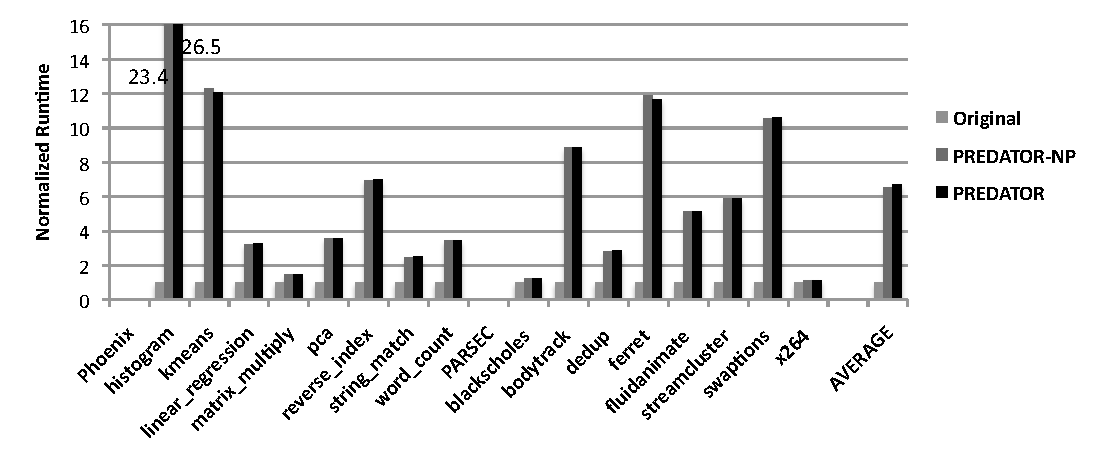
\includegraphics[width=6in]{predator/figure/perf}
\caption{
Performance overhead of \Predator{} with and without prediction(PREDATOR-NP).
\label{fig:perf}}
\end{figure*}

To avoid the effect caused by extreme outliers, all performance data shown in Figure~\ref{fig:perf} is based on the average of $10$ runs, excluding the maximum and minimum values. 

For $16$ benchmarks from the Phoenix and PARSEC benchmark suites and six real applications, \Predator{} imposes $5.4\times$ performance overhead. There is no noticeable difference on performance whether the prediction mechanism is enabled or not. 
 
Among these programs, five of them, histogram, kmeans, bodytrack, ferret, and swaptions, have more than $8\times$ performance overhead. The histogram benchmark runs more than $26\times$ slower than original executions with \pthreads{} library, because tracking detailed access on cache lines with false sharing exacerbates the false sharing effect (see more discussion in Section~\ref{sec:sample}).  For bodytrack and ferret, although there is no false sharing, \Predator{} detects a large amount of cache lines with writes larger than {\it Tracking-Threshold}. Thus, tracking those accessing details for those cache lines imposes significant performance overhead. Currently, we cannot identify the reasons why kmeans runs very slowly on \Predator{}.
   
\Predator{} imposes a small performance overhead for IO-bound applications, such as matrix\_multiply, blackscholes, x264, aget, Memcached, pbzip2, and pfscan, since \Predator{} does not add any performance overhead for IO operations.  

\subsection{Memory Overhead}
\label{sec:memoverhead}
We only evaluate the physical memory overhead of \Predator{}, instead of the virtual memory overhead, because \Predator{} allocates four gigabytes virtual memory for its custom memory allocator. Proportional set size (PSS) in \texttt{/proc/self/smaps} reflects the physical memory increase on the existing system of running an application~\cite{memusage}. Thus, we periodically collect this data and use the sum of different memory mappings as the total physical memory usage of running an application. We present the maximum value of physical memory usage in Figure~\ref{fig:memusage}. 

\Predator{} imposes less than 50\% memory overhead for 17 out of 22 applications.  For swaptions and aget, \Predator{} introduces more memory overhead because the original memory footprints of them are very small, only $3$ kilobytes. Adding the code of detection, prediction and reporting contributes to a large ratio of memory overhead. We are not clear why MySQL consumes much more memory than others. Although the average memory usage of all applications is over $2\times$, the total memory usage overhead is only about $40\%$ on \Predator{}. 


\subsection{Sensitivity to Different Sampling Rates}
\label{sec:sensitivity}
In Section~\ref{sec:sample}, we discuss that \Predator{} utilizes the sampling mechanism to reduce the tracking overhead. Running an application with different sampling rates does not affect its memory usage. Thus, we only evaluate the effect of different sampling rates on performance and effectiveness. 

The default sampling rate used by \Predator{} is 1\%. In this section, we also evaluate two other sampling rates, 0.1\% and 10\%. The performance results under the three different sample rates are shown in Figure~\ref{predator/figure:sample}. \Predator{} introduces less performance overhead under a lower sampling rate, which meets our expectation. Concerning effectiveness, even using the 0.1\% sampling rate, \Predator{} can still detect all false sharing problems, but with a lower number of cache invalidations. Thus, different sampling rates do not affect the detection effectiveness.
 
\begin{figure*}[!t]
\centering
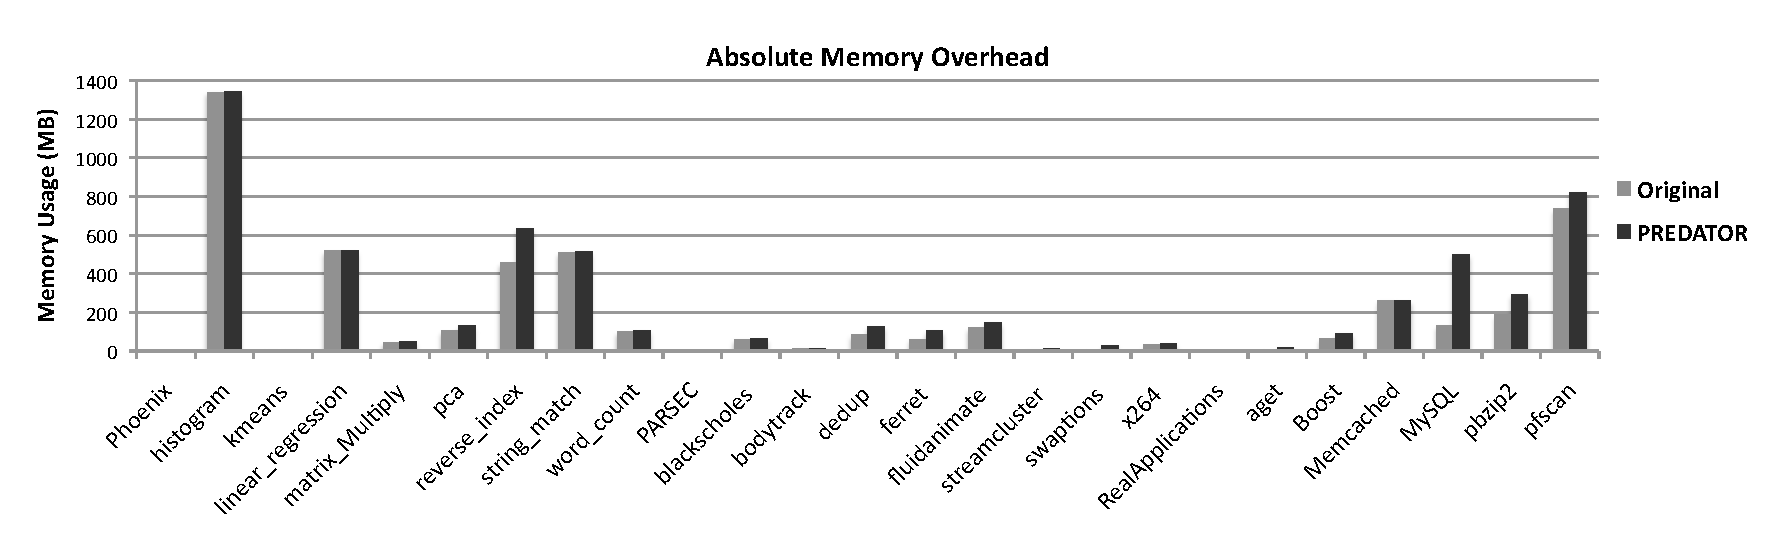
\includegraphics[width=6in]{predator/figure/absolutememory}
\caption{Absolute physical memory usage overhead with \Predator{}.}
\label{fig:absolutememusage}
\end{figure*}

\begin{figure*}[!t]
\centering
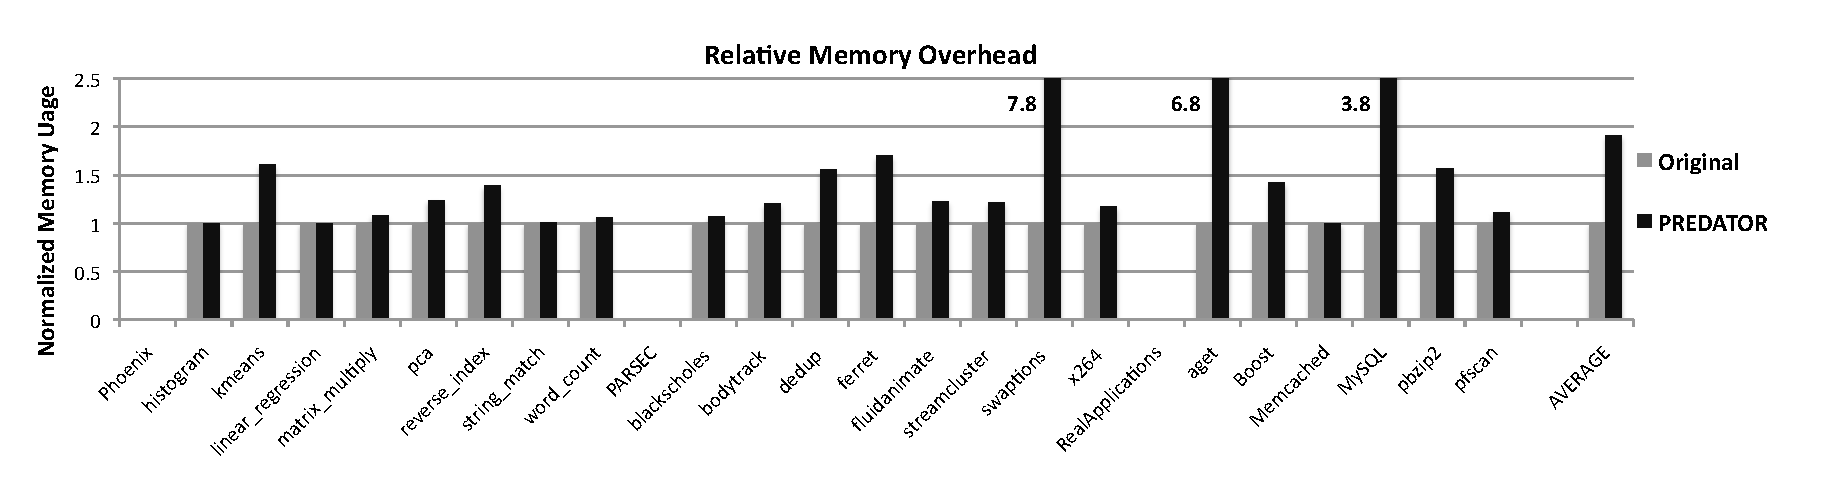
\includegraphics[width=6in]{predator/figure/memusage}
\caption{Relative physical memory usage overhead with \Predator{}.}
\label{fig:memusage}
\end{figure*}



\section{Related Work}

\label{chapter:relatedwork}
This chapter first describes those related work to processes-as-threads framework and deterministic execution. Then it describes related work in false sharing detection, prevention, or both. 

\section{Processes-As-Threads framework}

BOP relies on strong isolation of processes to automatically and safely parallelize the execution of programs~\cite{DingBOP}. BOP forks a new process to do speculation, based on those pre-defined possibly parallel regions (PPR). In order to check the correctness, BOP tracks accesses on a page-based granularity. When there is no conflict and a speculative process reaches the end of its current PPR, its predecessor always commits its changes to the current process. However, BOP does not provide any synchronization support and can not be used to run normal multithreaded programs. 

Grace is a process-based approach designed to prevent
concurrency errors, such as deadlock, race conditions, and
atomicity errors by imposing a sequential semantics on
speculatively-executed threads~\cite{grace}. Grace supports only fork-join programs without inter-thread communication (e.g., condition variables or barriers), and rolls back threads when accesses of threads would violate sequential semantics: a thread accesses pages that have been accessed by its predecessors. Grace can not support arbitrary multithreaded programs. Similar to the Grace system, Sammati is a processes-as-threads system to detect and tolerate deadlock problems~\cite{Pyla:2010:ADA:1854273.1854288}. However, Sammati does not support the full range of synchronizations, without synchronizations, barriers, and signals. Also, Semmati can not avoid race conditions happening in creating twin pages, which are avoided by \Sheriff{} framework.

\begin{comment}
% Some usage of this framework
According to Revisions,  Grace cannot easily resolve all
conflicts on commit (like revisions do) and must thus restrict
tasks from producing such conflicts either statically (by type
system) or dynamically (pessimistic with blocking, or optimistic with abort and retry). Also, Grace allows only a restricted “fork-join” form of concurrency
Revisions~\ref{Burckhardt:2010:CPR:1869459.1869515}
\end{comment}

\section{Deterministic Multithreading}
The research on deterministic multithreading is a very active area these years. We describe some software-only, non- language-based approaches here.

\subsection{Software-only deterministic system}
Grace prevents deadlocks, race conditions, ordering and atomicity violations errors for those fork-join multithreaded programs by imposing a sequential semantics at join points~\cite{grace}. However, Grace does not support programs with interthread communications, such as conditional variables and barriers.

CoreDet is a compiler-based approach to 
support general-purpose multithreaded programs~\cite{Bergan:2010:CCR:1736020.1736029}. 
CoreDet instruments those memory read and write operations as long
as those operations can not be proved to be thread-local in static analysis. 
In the runtime phase, CoreDet divides the execution into 
alternating parallel and serial phases and guides all memory operations 
using a memory ownership table: only those owned locations can be accessed
in the parallel phases; all non-owned locations and synchronizations can only 
be accessed in the serial phases guided by a global token.
CoreDet guarantees deterministic execution for racy programs without memory errors,
but with very high performance overhead: 
averagely $3.5\times$ slower than those using \pthreads{} library.
In order to guarantee determinsim, 
CoreDet has to serialize \emph{all} external library calls without instrumentation.
CoreDet doesn not provide deterministic 
memory allocations, which can not guarantee determinism for programs with memory errors.  
% The use of synchronization points as commit boundaries also makes \dthreads{}
% code relatively \emph{robust}: when updates occur after a given number of 
% instructions retired (as in CoreDet and Kendo), it is impossible for 
% programmers to know when interleavings can occur. Such boundaries could vary 
% depending on the underlying architecture and would also be input-dependent, 
% meaning that slightly different inputs could lead to dramatically different
% thread interleavings. By contrast, \dthreads{} guarantees that only changes to
% the sequence of synchronization operations affect the order in which updates 
% are applied.
dOS~\cite{deterministic-process-groups} is an extension to CoreDet
that uses the same deterministic scheduling framework.  dOS 
supports deterministic communication for those threads and processes inside the same
deterministic process groups (DPGs) and handle those external non-determinism by recording and
replaying interactions across DPG boundaries. 

Determinator is a microkernel-based operating system that enforces
system-wide determinism~\cite{efficient-system-enforced}.
Determinator provides separate address spaces and supports interprocess
communications at explicit synchronizaton points. 
Determinator is a proof-of-concept system, which can not support the whole rage of
threads APIs and can not work on legacy programs.  

Some other works can only support limited determinism or need user annotation.
Kendo can only guarantee the determinism for race-free programs~\cite{1508256}. 
TERN~\cite{stable-deterministic} provides a best-effort system to 
apply memoized schedules for future runs with similar inputs. 
It can not guarantee the determinism for racy programs, as Kendo. 
Peregrine~\cite{peregrine:sosp11} is a system based on TERN, which tries to record
 memory accesses orders for racy portion and apply those schedules for future runs possibly.
However, both TERN and Peregrine do not support complete determinism (using a best effort)
and requires program annotations. 

\subsection{Hardware-related deterministic System}

\section{False Sharing}

This section describes related work in false sharing detection, prevention, or both. There is no previous
system to predict unobserved false sharing.

\subsection{False Sharing Detection}
Based on the SIMICS functional simulator, Schindewolf et al.\ designed a tool to report different kinds of cache usage information, such as cache misses and cache invalidations~\cite{falseshare:simulator}. Pluto relies on Valgrind dynamic instrumentation framework to track the sequence of memory read and write events on different threads, and reports a worst-case estimation of possible false sharing~\cite{falseshare:binaryinstrumentation1}.
Similarly, Liu uses Pin to collect memory access information, and reports total cache miss information~\cite{falseshare:binaryinstrumentation2}.
These tools impose about $100-200\times$ performance overhead.

Zhao et al.\ developed a tool based on DynamoRIO framework to detect false sharing and other cache contention problems
for multithreading programs~\cite{qinzhao}. 
It uses a shadow memory technique to maintain memory access history and detects cache invalidations based on the ownership of cache lines. However, it can only support at most $8$ threads. In addition, it cannot differentiate cold cache misses from actual false sharing problems.

Intel's performance tuning utility (PTU) uses Precise Event Based Sampling (PEBS) hardware support to detect false sharing problems ~\cite{detect:ptu, detect:intel}.  PTU cannot distinguish true sharing from false sharing. In addition, PTU aggregates memory accesses without considering memory reuses and access interleaving, leading to numerous false positives. Sanath et al. designed a machine learning based approach to detect false sharing problems. They train their classifier on mini-programs and apply this classifier to general programs ~\cite{mldetect}. Instead of instrumenting memory accesses, this tool relies on hardware performance counters to collect memory accesses events. It achieves very low performance overhead(about 2\%). But it relies on hardware support for its efficiency.  

In addition to their individual disadvantages,
all approaches discussed above share a common shortcoming:  
they cannot pinpoint the exact location of false sharing in the source code, so programmers have to examine the source code and identify problems manually.

Pesterev et al.\ present DProf, a tool that help programmers identify cache misses based on AMD's instruction-based sampling hardware~\cite{DProf}. DProf requires manual annotation to locate data types and object fields, and cannot detect false sharing when multiple objects reside on the same cache line.

\subsection{False Sharing Prevention}
\label{sec:fspreventwork}
% More approaches
Jeremiassen and Eggers use a compiler transformation to automatically adjust the memory layout of applications through padding and alignment~\cite{falseshare:compile}. Chow et al.\ alter parallel loop scheduling in order to avoid false
sharing~\cite{falseshare:schedule}. These approaches only works for regular, array-based scientific code.

Berger et al.\ describe Hoard, a scalable memory allocator that can reduce the possibility of false sharing by making different threads use different heaps~\cite{Hoard}. Hoard cannot avoid false sharing problem in global variables or within
a single heap object: the latter appears to be the primary source of real false sharing problems.

\subsection{False Sharing Detection and Prevention}

Plastic leverages the sub-page granularity memory remapping facility provided by the Xen hypervisor to detect and tolerate false sharing automatically~\cite{OSdetection}. However, the sub-page memory remapping mechanism is not currently supported by most existing operating system, reducing its generality. In addition, Plastic cannot pinpoint the exact source of false sharing.  
In order to utilize Plastic's prevention tool, a program has to run on the Xen hypervisor, limiting the applicability of their prevention technique.



\section{Future Work}
\label{sec:future}
\label{futurework}

We plan to extend \sheriff{} to find more performance related problems in
multithreaded programs. For example, if one frequently-read word
happens to be in the same cache line with one frequently-written word,
it would be better to separate those two words. But in the current
framework, \sheriff{} cannot detect a single memory read operation using the
twin page mechanism. We are examining the combination of hardware
watchpoints to help us locate this kind of performance error. In
addition, we plan to exploit watchpoints to capture those program
counters that touch specific addresses so as to point the programmer
to specific lines of code responsible for false sharing.



\label{sec:future}
\begin{comment}
(1) Pinpoint the line number to access the cache line by using the "watch point" technique. \\
(2) Figure out the problem caused by read-write false sharing problem by using the "watch point" technique. \\
(3) Design a run-time system which can tolerate the false sharing problem in a very low overhead. Profiling
on specified input should be very helpful to find the problem.
\end{comment}

\section{Conclusion}
\label{sec:conclusion}

\dthreads{} is a deterministic replacement for the \pthreads{}
library that supports general-purpose multithreaded
applications. \dthreads{} is straightforward to deploy, requiring no
source code, and operates on commodity hardware. By converting threads
into processes, \dthreads{} leverages process isolation and virtual
memory protection to track and isolate concurrent memory updates with
low overhead. By committing these changes deterministically at natural
synchronization points in the code, rather than at boundaries based on
hardware performance counters, \dthreads{} not only ensures full
internal determinism---eliminating data races as well as
deadlocks---but does so in a way that is portable and easy to
understand. Its software architecture prevents false sharing, a
notorious performance problem for multithreaded applications running
on multiple, cache-coherent processors. The combination of these
approaches enables \dthreads{} to match or even exceed the performance
of \pthreads{} for the majority of the benchmarks examined here,
making \dthreads{} a safe and efficient alternative to \pthreads{} for
some applications.

{
% \footnotesize
\small
\bibliographystyle{abbrv}
\bibliography{ref,emery}
}

\end{document}
